\documentclass{report}

\input{~/dev/latex/template/preamble.tex}
\input{~/dev/latex/template/macros.tex}

\title{\Huge{}}
\author{\huge{Nathan Warner}}
\date{\huge{}}
\pagestyle{fancy}
\fancyhf{}
\lhead{Warner \thepage}
\rhead{}
% \lhead{\leftmark}
\cfoot{\thepage}
%\setborder
% \usepackage[default]{sourcecodepro}
% \usepackage[T1]{fontenc}

\begin{document}
    % \maketitle
        \begin{titlepage}
       \begin{center}
           \vspace*{1cm}
    
           \textbf{Calculus II} \\
           Chapter 2: Applications of Integration
    
           \vspace{0.5cm}
            
                
           \vspace{1.5cm}
    
           \textbf{Nathan Warner}
    
           \vfill
                
                
           \vspace{0.8cm}
         
           \includegraphics[width=0.4\textwidth]{~/niu/seal.png}
                
           Computer Science \\
           Northern Illinois University\\
           September 08, 2023 \\
           United States\\
           
                
       \end{center}
    \end{titlepage}
    \tableofcontents
    \pagebreak \bigbreak \noindent
    \vspace{2in} \\
    \begin{Huge}
        \textbf{Applications \\ of Integration}
    \end{Huge}
    \bigbreak \noindent 
    \line(1,0){490}
    \bigbreak \noindent 
    \section*{\LARGE 2.1: Areas between Curves}
    \addcontentsline{toc}{section}{2.1: Areas between Curves}
    \bigbreak \noindent 
    \phantomsection
    \addcontentsline{toc}{subsection}{Area of a Region between Two Curves}
    \subsection*{Area of a Region between Two Curves}
    Let \( f(x) \) and \( g(x) \) be continuous functions over an interval \([a,b]\) such that \( f(x) \geq g(x) \) on \([a,b]\). We want to find the area between the graphs of the functions, as shown in the following figure.
    \bigbreak \noindent 
    \begin{center}
        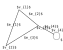
\includegraphics[scale=.5]{./figures/graph1.png  }
    \end{center}
    \bigbreak \noindent 
    As we did before, we are going to partition the interval on the \( x \)-axis
    and approximate the area between the graphs of the functions with rectangles. So, for \( i=0,1,2,\ldots,n \),
    let \( P = \{ x_i \} \)
    be a regular partition of \( [a,b] \).
    Then, for \( i=1,2,\ldots,n \),
    choose a point \( x^*_i \in [x_{i-1}, x_i] \),
    and on each interval \( [x_{i-1}, x_i] \)
    construct a rectangle that extends vertically from \( g(x^*_i) \)
    to \( f(x^*_i) \).
    Figure 2.3(a) shows the rectangles when \( x^*_i \)
    is selected to be the left endpoint of the interval and \( n=10 \).
    \begin{center}
        \includegraphics[scale=0.5]{ ./figures/2aaddefc-a60a-41ed-8312-ef6960ad3b6c.png }
    \end{center}
    \pagebreak \bigbreak \noindent 
    The height of each individual rectangle is \( f(x^*_i) - g(x^*_i) \) and the width of each rectangle is \( \Delta x \).
    Adding the areas of all the rectangles, we see that the area between the curves is approximated by

    \[
    A \approx \sum_{i=1}^{n} \left[ f(x^*_i) - g(x^*_i) \right] \Delta x.
    \]
    \bigbreak \noindent 
    This is a Riemann sum, so we take the limit as \( n \to \infty \) and we get
    \[
    A = \lim_{{n \to \infty}} \sum_{i=1}^{n} \left[ f(x^*_i) - g(x^*_i) \right] \Delta x = \int_{a}^{b} \left[ f(x) - g(x) \right] \, dx.
    \]
    \bigbreak \noindent 
    These findings are summarized in the following theorem.
    \bigbreak \noindent 
    \begin{thrm}
       Let \( f(x) \) and \( g(x) \) be continuous functions such that \( f(x) \geq g(x) \) over an interval \([a, b]\).
Let \( R \) denote the region bounded above by the graph of \( f(x) \), below by the graph of \( g(x) \), and on the left and right by the lines \( x = a \) and \( x = b \), respectively. Then, the area of \( R \) is given by

    \[
    A = \int_{a}^{b} \left[ f(x) - g(x) \right] \, dx.
    \] 
    \end{thrm}
    \bigbreak \noindent 
    Quite often, though, we want to define our interval of interest based on where the graphs of the two functions intersect. This is illustrated in the following example.
    \smallbreak \noindent
    \begin{eg}
       If \( R \) is the region bounded above by the graph of the function \( f(x) = 9 - \left( \frac{x}{2} \right)^2 \) and below by the graph of the function \( g(x) = 6 - x \), find the area of region \( R \).
    \end{eg}
    \bigbreak \noindent \bigbreak \noindent 
    \begin{minipage}{0.47\textwidth}
    \begin{center}
        \includegraphics[scale=.35]{ ./figures/graph3.png}
    \end{center}
    \end{minipage}
    \begin{minipage}{0.47\textwidth}
        To find our limits of integration, we first need to find where the two functions intersect.
        \begin{align*}
            &=9 - \bigg(\frac{x}{2}\bigg)^{2} = 6-x \\
            &=9 - \frac{x^{2}}{4} = 6-x \\
            &=\frac{36-x^{2}}{4} = 6-x \\
            &= 36 -x^{2} = 24-4x \\
            &= -x^{2} +4x +12 \\
            &= -(x^{2}-4x-12) = 0 \\
            &= -(x-6)(x+2) \\
            &= x=6,-2
        .\end{align*}
        Thus, we need to integrate from x=-2 to 6
        \bigbreak \noindent 
    \end{minipage}
    \smallbreak \noindent
    By Theorem 1: $A = \int_{a}^{b}\ \big[f(x)-g(x)\big]\ dx $, we find that:
    \begin{align*}
        A = \frac{64}{3}\ Units^{2}
    .\end{align*}

    \pagebreak \bigbreak \noindent 
    \phantomsection
    \addcontentsline{toc}{subsection}{Areas of Compound Regions}
    \subsection*{Areas of Compound Regions}
    \bigbreak \noindent 
    So far, we have required  $f(x) \geq g(x)$ over the entire interval of interest, but what if we want to look at regions bounded by the graphs of functions that cross one another? In that case, we modify the process we just developed by using the absolute value function.
    \bigbreak \noindent 
    \begin{thrm}
        Let \( f(x) \) and \( g(x) \) be continuous functions over an interval \([a, b]\).
        Let \( R \) denote the region between the graphs of \( f(x) \) and \( g(x) \),
        and be bounded on the left and right by the lines \( x = a \) and \( x = b \), respectively.
        Then, the area of \( R \) is given by
       \begin{align*}
          \int_{a}^{b}\ \abs{f(x)-g(x)}\ dx 
       .\end{align*} 
    \end{thrm}
    \bigbreak \noindent 
    In practice, applying this theorem requires us to break up the interval [a,b] and evaluate several integrals, depending on which of the function values is greater over a given part of the interval. We study this process in the following example.
    \bigbreak \noindent 
    \begin{eg}
       If \( R \) is the region between the graphs of the functions \( f(x) = \sin x \) and \( g(x) = \cos x \) over the interval \([0, \pi]\), find the area of region \( R \).
    \end{eg}
    \bigbreak \noindent 
    \begin{minipage}{0.47\textwidth}
        \begin{center}
            \includegraphics[scale=0.5]{./figures/51be43c1-417e-4df2-a3d0-7d6ec562ccb2.png}
        \end{center}
    \end{minipage}
    \begin{minipage}{0.47\textwidth}
        By theorem 2, we can find the area $A$, in the region $R$ with the following integral:
        \begin{align*}
            &\int_{a}^{b}\ \abs{f(x)-g(x)}\ dx \\
            &=\int_{0}^{\pi}\ \abs{\sin{x}-\cos{x}}\ dx \\
        .\end{align*}
        First, we need to find where the sign of the expression changes:
        \begin{align*}
            &=\sin{x} - \cos{x} = 0 \\
            &=\frac{\sin{x}}{\cos{x}} = \frac{\cos{x}}{\cos{x}} \\
            &=\tan{x} = 1 \\
            &x = \tan^{-1}{1},\ \quad \bigg(-\frac{\pi}{2},\frac{\pi}{2}\bigg) \\
            &x= \frac{\pi}{4}
        .\end{align*}
    \end{minipage}
    \pagebreak \bigbreak \noindent 
    \begin{minipage}{0.47\textwidth}
        Thus:
           \begin{equation}
            \sin{x} - \cos{x}=
                \begin{cases}
                     \sin{x}-\cos{x}& \text{if } x \geq \frac{\pi}{4} \\
                     -(\sin{x}-\cos{x})& \text{if } x < \frac{\pi}{4} 
                \end{cases}
            \end{equation}
    \end{minipage}
    \begin{minipage}[t]{0.47\textwidth}
        So our integral is now:
        \begin{align*}
            &\int_{0}^{\frac{\pi}{4}}\ -(\sin{x}-\cos{x}) dx + \int_{\frac{\pi}{4}}^{\pi}\ \sin{x}-\cos{x}\ dx \\
            &=\int_{0}^{\frac{\pi}{4}}\ \cos{x}-\sin{x}\ dx + \int_{\frac{\pi}{4}}^{\pi}\ \sin{x}-\cos{x}\ dx \\
            &Where:\ I_{1} = \int_{0}^{\frac{\pi}{4}}\ \cos{x}-\sin{x}\ dx \\
            &I_{2} = \int_{\frac{\pi}{4}}^{\pi}\ \sin{x}-\cos{x}\ dx \\
            &A = I_{1} + I_{2}
        .\end{align*}
    \end{minipage}
    \bigbreak \noindent 
    \begin{minipage}[t]{0.47\textwidth}
        Computing both integrals we get:
    \end{minipage}
    \begin{minipage}[t]{0.47\textwidth}
    
    \begin{align*}
        &I_{1} = \int_{0}^{\frac{\pi}{4}}\ \cos{x}-\sin{x}\ dx \\
        &=\sin{x} + \cos{x}\bigg]^{0}_{\frac{\pi}{4}} \\
        &= \bigg(\sin{\bigg(\frac{\pi}{4}\bigg)+\cos{\bigg(\frac{\pi}{4}\bigg)}}\bigg) - \bigg(\sin{(0)+\cos{0}}\bigg)\\
        &= \sqrt{2} - 1
    .\end{align*}
    \begin{align*}
        &=I_{2} = \int_{\frac{\pi}{4}}^{\pi}\ \sin{x}-\cos{x}\ dx \\
        &= -\cos{x}-\sin{x}\bigg]^{\frac{\pi}{4}}_{\pi} \\
        &= - \bigg[\cos{x}+\sin{x}\bigg]^{\pi}_{\frac{\pi}{4}} \\
        &= - \bigg[\bigg(\cos{\pi}+\sin{\pi}\bigg) - \bigg(\cos{\bigg(\frac{\pi}{4}\bigg)+\sin{\bigg(\frac{\pi}{4}\bigg)}}\bigg)\bigg] \\
        &= - \bigg[-1 - \sqrt{2}\bigg] \\
        &= 1 + \sqrt{2}
    .\end{align*}
    \end{minipage}
    \bigbreak \noindent 
    \begin{minipage}[t]{0.47\textwidth}
        Thus:
    \end{minipage}
    \begin{minipage}[t]{0.22\textwidth}
        \begin{align*}
        &A = I_{1} + I_{2} \\
        &= \sqrt{2} - 1 + 1 + \sqrt{2} \\
        & = 2\sqrt{2}\ \ \ Units^{2}
    .\end{align*}
    \end{minipage}

    \pagebreak 
    \phantomsection
    \addcontentsline{toc}{subsection}{Finding the Area of a Complex Region}
    \subsection*{Finding the Area of a Complex Region}
    \smallbreak \noindent
    \begin{definition}
    \textbf{a "complex region" between curves usually refers to an area that is not easily described by a single, continuous function over the interval of interest.} 
    \end{definition}
    \bigbreak \noindent 
    Consider the following example:
    \smallbreak \noindent
    \begin{eg}
        If \( R \) is the region between the graphs of the functions \( f(x) = x^{2} \) and \( g(x) = 2-x \) over the interval \([0, 2]\), find the area of region \( R \).
    \end{eg}
    \bigbreak \noindent 
    \begin{minipage}{0.47\textwidth}
        \bigbreak \noindent 
        \textit{Figure 2.7}
        \begin{center}
            \includegraphics[scale=0.7]{ ./figures/graph4.png }
        \end{center}
    \end{minipage}
    \begin{minipage}{0.47\textwidth}
        As with Example 2.3, we need to divide the interval into two pieces. The graphs of the functions intersect at \( x=1 \) (set \( f(x)=g(x) \) and solve for \( x \)), so we evaluate two separate integrals: one over the interval \([0,1]\) and one over the interval \([1,2]\).
        \bigbreak \noindent 
        Over the interval \([0,1]\), the region is bounded above by \( f(x)=x^2 \) and below by the x-axis, so we have
        \[
        A_1 = \int_{0}^{1} x^2 \, dx = \left. \frac{x^3}{3} \right|_{0}^{1} = \frac{1}{3}.
        \]

        Over the interval \([1,2]\), the region is bounded above by \( g(x)=2-x \) and below by the x-axis, so we have
        \[
        A_2 = \int_{2}^{1} (2-x) \, dx = \left[ 2x - \frac{x^2}{2} \right]_{2}^{1} = \frac{1}{2}.
        \]

        Adding these areas together, we obtain
        \[
        A = A_1 + A_2 = \frac{1}{3} + \frac{1}{2} = \frac{5}{6}.
        \]
        The area of the region is \( \frac{5}{6} \) \text{units}^2.
    \end{minipage}

    \pagebreak
    \phantomsection
    \addcontentsline{toc}{subsection}{Regions Defined with Respect to y}
    \subsection*{Regions Defined with Respect to y}
    \bigbreak \noindent 
    In Example 3, we had to evaluate two separate integrals to calculate the area of the region. However, there is another approach that requires only one integral. What if we treat the curves as functions of \( y \), instead of as functions of \( x \)?
    \bigbreak \noindent 
    Review Figure 2.7. Note that the left graph, shown in red, is represented by the function \( y = f(x) = x^2 \).
    We could just as easily solve this for \( x \) and represent the curve by the function \( x = v(y) = \sqrt{y} \).
    \bigbreak \noindent 
    \nt{(Note that \( x = -\sqrt{y} \) is also a valid representation of the function \( y = f(x) = x^2 \) as a function of \( y \). However, based on the graph, it is clear we are interested in the positive square root.)}
    \bigbreak \noindent 
    Similarly, the right graph is represented by the function \( y = g(x) = 2 - x \), but could just as easily be represented by the function \( x = u(y) = 2 - y \).
    \bigbreak \noindent 
    When the graphs are represented as functions of $y$, we see the region is bounded on the left by the graph of one function and on the right by the graph of the other function. Therefore, if we integrate with respect to $y$, we need to evaluate one integral only. Let’s develop a formula for this type of integration.
    \bigbreak \noindent \bigbreak \noindent  
    \begin{minipage}{0.47\textwidth}
        \begin{center}
            \includegraphics[scale=0.6]{./figures/graph5.png}
        \end{center}
    \end{minipage}
    \begin{minipage}{0.47\textwidth}
        Let \( u(y) \) and \( v(y) \) be continuous functions over an interval \([c, d]\) such that \( u(y) \geq v(y) \) for all \( y \in [c, d] \). We want to find the area between the graphs of the functions, as shown in the following figure.
    \end{minipage}
    \bigbreak \noindent 
    \begin{minipage}{0.47\textwidth}
        \bigbreak \noindent 
        \textit{Figure 2.9}
        \begin{center}
            \includegraphics[scale=.45]{./figures/graph6.png }
        \end{center} 
    \end{minipage}
    \begin{minipage}{0.47\textwidth}
        This time, we are going to partition the interval on the \( y \)-axis and use horizontal rectangles to approximate the area between the functions. So, for \( i = 0, 1, 2, \ldots, n \), let \( Q = \{ y_i \} \) be a regular partition of \([c, d]\). Then, for \( i = 1, 2, \ldots, n \), choose a point \( y^*_i \in [y_{i-1}, y_i] \), then over each interval \([y_{i-1}, y_i]\) construct a rectangle that extends horizontally from \( v(y^*_i) \) to \( u(y^*_i) \).
    %\caption{}
    %\label{fig:}
    \end{minipage}
    \bigbreak \noindent 
    \nt{Figure 2.9(a) shows the rectangles when \( y^*_i \) is selected to be the lower endpoint of the interval and \( n = 10 \).
        Figure 2.9(b) shows a representative rectangle in detail.
}
    \pagebreak \bigbreak \noindent 
    The height of each individual rectangle is \( \Delta y \) and the width of each rectangle is \( u(y^*_i) - v(y^*_i) \). Therefore, the area between the curves is approximately
    \[
    A \approx \sum_{i=1}^{n} [u(y^*_i) - v(y^*_i)] \Delta y
    \]
    This is a Riemann sum, so we take the limit as \( n \to \infty \), obtaining
    \[
    A = \lim_{{n \to \infty}} \sum_{i=1}^{n} [u(y^*_i) - v(y^*_i)] \Delta y = \int_{c}^{d} [u(y) - v(y)] \, dy
    \]
    These findings are summarized in the following theorem.
    \bigbreak \noindent 
    \begin{thrm}
       Let \( u(y) \) and \( v(y) \) be continuous functions such that \( u(y) \geq v(y) \) for all \( y \in [c, d] \). Let \( R \) denote the region bounded on the right by the graph of \( u(y) \), on the left by the graph of \( v(y) \), and above and below by the lines \( y = d \) and \( y = c \), respectively. Then, the area of \( R \) is given by
        \[
        A = \int_{c}^{d} [u(y) - v(y)] \, dy
        \] 
    \end{thrm}

    \pagebreak 
    \phantomsection
    \addcontentsline{toc}{section}{2.2 Determining Volumes by Slicing}
    \section*{2.2 Determining Volumes by Slicing}
    \bigbreak \noindent 
    




    


    

\end{document}
